\section{Components}
%The functionality of the bus has been split into four components, that can be designed, implemented and tested independently. The following section will describe the components in this section. Additionally, the tracks will be tested using tracks designed specifically to test whether the components conform to the individual requirements \ref{Requirements}.

%This section lists the different prototypes with their design, purpose, and objectives that it needs to fulfil in order to be a completed prototype. Furthermore, it will describe the tracks that are designed for testing the functionality of each prototype. The prototypes will take base from the requirements in section \ref{Requirements}.

The functionality of the bus has been split into four components of functionality, which can be implemented and tested independently. They do require basic driving functionality, however. For this reason, we first implement the \code{Driving} component along with the \code{MotorController}, and then the following components. As we implement the components of functionality thereafter, we test the bus on a track specifically tailored to challenge that functionality. The creation of these tracks will also be recounted. 

\subsection{Driving Component}

\section{StayWithinLane}

In this section we describe the implementation of the StayWithinLane-component and the NxtCamLineTrackController. We begin with the controller for the nxtCamV4, as it is essential for the StayWithinLane component to work. 

\subsection{NxtCamLineTrackController}

The point of the controller is that we can call it to get the coordinates of the lines that have been detected by the camera sensor without having to worry about any NxtCam sensor specifics or behind the scenes calculations. 

When called in line tracking mode, the NxtCam returns between 0 and 8 objects with corresponding height, width and position of a slice of a detected line. A number of data manipulations must now be performed in order to convert these points from the cameras local space \ref{Measure With NxtCam} into a new 2 dimensions local space with origin in the NxtCam position \ref{??}. The coordinates in this space correspond with the real world based on where is NxtCam is in world space, so the distance can be calculated. The intent is that we can use the clean data points to calculate the direction which the bus must drive in order to stay in the middle of the road. 

The steps that are performed to clean up the NxtCam measurements and their return values are written in order: 


\begin{description}
    \item[Measure With NxtCam]
    Raw measurements from the nxtCam. The camera starts mapping in the top-left corner (coordinate 0,0) down to the bottom-right (coordinate 144,176).
    \item[Displace and Flip Coordinate Plot]
    Moves the origin of plot to the bottom-middle (coordinate 0,88) where the camera is placed and flips the x-coordinates. As such, the top-left becomes coordinate 144,-88 and the bottom-right point becomes coordinate 144,88. 
    \item[Correct for Lens Distortion]
    The bend of the camera lens distorts the position of points in regards to where they are actually placed. This is corrected in this function. 
    \item[Sort Out Bad Measurements]
    Any measurements that are not placed within either the left or right road markings are sorted out. 
    \item[Correct for Field of View]
    The coordinates and distances between points are incorrect because the picture was taken at an angle, and as such the objects at the top are further away from the camera than the objects at the bottom of the picture. This is corrected in this function. 
\end{description}

%(Ren punktdata) NxtCamV4 Line Tracking Driver: Track Line ()
%	(Rå punktdata) Mål med NxtCamV4 ()
%	(Rykket koordinatsystem) Flyt og vend koordinatsystem (Rå punktdata)
%	*(Let modificeret punktdata) Funktion for distortion (Rykket punktdata)
%	*(Ren punktdata) Funktion der sorterer dårlige målinger fra (Let modificeret punktdata)			- Målinger der ligger helt forkert, for eksempel
%	(Punkter på koordinatsystem) NxtCamV4 Line Tracking Driver: Map Points to Koordinates (Ren punktdata)
%	- Property: Bus Point


\subsubsection{Field of View Corrections}
See appendix \ref{fieldOfViewCorrections} for our algorithm to correct for field of view. The rest of the steps in the NxtCamLineTrackController will not be described in more detail. The algorithm for field of view was translated into C++ as the class FieldOfViewCorrector where it works as described in the document. 

The values given for the field of view corrections are not fixed, meaning that the camera can be moved higher, lower and tilted towards or away from the ground without causing issues in regards to these calculations. 

\subsection{Algorithm}
In this section the algorithm that ensures that the bus always stays within the road lane is described. 

The intent for the algorithm is to calculate an optimal line that the bus should follow in order to keep within lane markings. Using this result, it will call the Driving-component and inform it how much the bus should turn its wheels and for how long with it's current speed. 

Before the points gained through the NxtCamLineTrackController can be used, they need to be sorted in left and right side. After this we calculate a bézier curve for each side to find a smooth midpoint line for the bus to follow. This is not quite as simple as it seems, as we need to handle the cases where the line tracker returns only very few points. For instance, if it returns only one coordinate for the left lane marking, then we cannot calculate a proper curve without knowledge of where at least one previous coordinate in the left lane was placed. 

To solve this, we save old measurements from the last time we calculated the path for the bus. However, these need to be moved along the x or y-axis to fit with the new position of the bus compared to the place where the old measurement took place. Additionally, these measurement will need to be rotated if the bus has driven part of a road curve since the last measurement. Also the bus will need to handle the case where there are zero measurement in the side. This is done by taking the measured point which is the farthest away, and the point previous to that in the same side. Next these two points are used to make a right-angle triangle so the farthest away point of the other side can me calculated \ref{fig:findK}. By doing this we get the point farthest away the camera can see in both sides. Now the bézier curves for both side will show approximately same length of the road. And that will make our calculation of midpoints between the two curves more accurate since the amount of points calculated on each bézier curves is a constant.

Now a constant of midpoints is calculated and the slope and length between each point is found. The slope tells the angle the bus needs to turn, if the slope is negative it means turn left, if positive turn right. And the length is the distance to be driven with the found slope. 


\begin{figure}[ht]
    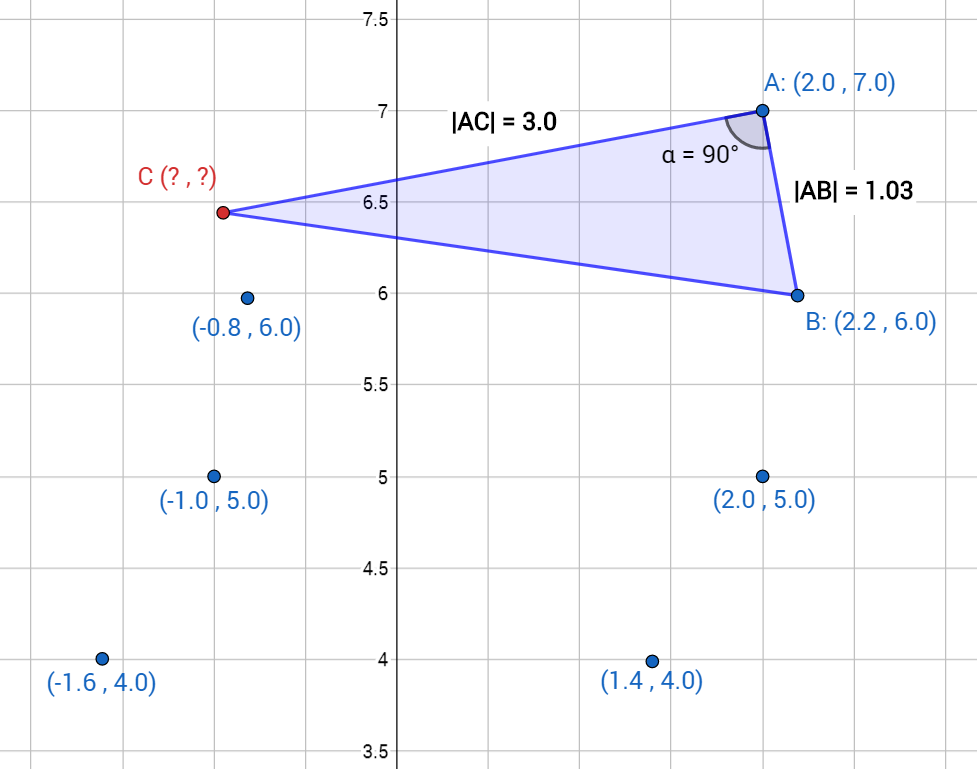
\includegraphics[width=\textwidth]{Images/Design/findK.PNG}
    \caption{Balance left/right data length.}
    \label{fig:findK}
\end{figure}




\begin{algorithm}[H]
 \KwData{this text}
 \KwResult{how to write algorithm with \LaTeX2e }
 initialization\;
 \While{not at end of this document}{
  read current\;
  \eIf{understand}{
   go to next section\;
   current section becomes this one\;
   }{
   go back to the beginning of current section\;
  }
 }
 \caption{How to write algorithms}
\end{algorithm}







\todo{Add the pictures I created for pineTreeProblem and lane correction over time}
%I feel like making the nxtCamLineTrack just return third order polynomials would have been better.

\begin{description}
    \item[NxtCamLineTrackController: Track Lines]
    Gets the cleaned coordinates from a picture using the previously described NxtCamLineTrackController class. 
    \item[Combine Old And New Coordinates]
    Combines old and new coordinates, moving and rotating the measurements to fit with the new position and wheel angle of the bus. 
    \item[Sort Data]
    Splits the coordinates into measurements belonging to the left and the right lane marking. 
    \item[Bézier Curve Calculation]
    A bézier curve is calculated for the left and right lane markings. Using this, a number of points in the middle of the road between the two bézier curves is calculated.
    \item[Calculate Driving Direction]
    Calculates which direction the bus should turn optimally. 
    \item[Call Driving Component]
    Calls the driving and informs it of the results.
\end{description}
\todo{1. LoadData, 2. Update Data to global space, 3. Sort New Data y and side, 4. Update OldData, 5. Combine Old and New data, 6. BezierCurves, 7. MidPoints, 8. Slope/Length.}

This algorithm has been implemented in the StayWithinLane-class of the program. \todo{We're in design, Can't write this!}
\todo{Describe part of code?}


%() Stay Within Lines: Algoritme ()- Basically, den kører prik-til-prik med midtpunkter
%	(Punkter på koordinatsystem) NxtCamV4 Line Tracking Driver: Track Line ()
%	(Gamle + Nye punkter på koordinatsystem) Sammensæt gammelt og nyt data ([Nye] Punter på koordinatsystem, Bus Point, [Gammel] Midpoint Bezier Curve)
%	(Sorteret Data Venstre, Sorteret Data Højre) Sorter Data (Gamle + Nye punkter på koordinatsystem)
%	(0-8 Midtpoints) Bezier Curve Udregning (Sorteret Data Venstre, Sorteret Data Højre)
%	*(Grader rotation, afstand der skal køres) Regn kørselsrute (0-8 Midtpoints)					- Hvis bussen ikke er i midten, skal den køre hen mod midtpoint. Håndterer også hvis den ikke får nok/nogle punkter

\subsection{ObstacleDetection}
%\section{BusStopDetection}
%\section{SpeedZoneDetection}





%\subsection{Staying Within the Lines}

\subsubsection{Component Requirements}
The requirements for this component are a reduced amount of the total requirements for the project.

From requirement 1, the component must be able to navigate a track constructed with the same relation between its width and the width of the bus as the \todo{Nej er først prototype.2}Danish Road Directorate dictates for Danish roads. This means the bus needs to drive, brake and turn. The bus' maximum turning radius only needs to be at least as much as the maximally allowed curve on Danish roads. 

As a less demanding requirement 4, the first component should avoid collisions with obstacles from the front. \unsure{The second requirement isn't strictly part of the steering "component", instead it's part of the overall bus prototype}

\subsection{Prototype Construction}
To create the component focused on steering the bus through the track, which will later be used in the final product, a prototype designed solely for this purpose is built. The prototype needs to be able to drive, turn and brake. Furthermore, it needs to be able to combine these mechanisms to stay within the lines of the track. A LEGO Servo Motor is connected to the rear wheels, which provides forwards and backwards movement capabilities. The speed consistency of the bus is not important in this prototype, however driving at a higher speed allows for testing the capabilities of the sensors and their processing speed.
%however the Servo Motor should be set at \todo{80\%}, to make sure the bus can drive at high speed and still stay within the lines at all times, but the actual speed are not to be measured.

\textbf{Turning}\newline
The front wheels are used for turning and is powered by a LEGO Servo Motor. It should be able to turn the same amount of degrees to both sides, however, there is no requirement for a specific turning angle for this prototype. A thing to note is that the track for the bus should be designed such that the bus can perform the turn within the lines.

\textbf{Obstacle Detection}\newline
To prevent crashes, the prototype supports obstacle detection by having a LEGO ultrasonic sensor mounted at the very front of the bus in a fixed position. The sensor detects obstacles up to 70 cm ahead and 30 degrees to both sides. If it predicts that a collision might occur, the bus stops immediately, overriding both the driving and turning procedures. When the obstacle is no longer a hindrance, it will return to its normal state.  % Later prototype should be able to get out of this situation

\textbf{Follow Track}\newline
For the prototype to stay within the lines of the track, a LEGO NXTCam-v4 should be placed at the front in the center. The sensor should be aimed at the ground in front of the bus in order to see the tracks.

The bus itself should be formed like a long rectangle so that it gets the form of a bus. It should have \todo{1:3?} length to width ratio.

\subsubsection{Track requirements}
The designed track for this prototype can be seen in figure \ref{Track1Layout}. The layout of the track is quite simple and only contain some of the requirements described in section \ref{Requirements}. The reason for this is to only test the features of this prototype and as such, it is designed uniquely for this prototype.

The requirements for the track has therefore been limited to:
\cite{DriveingCurves}
\begin{itemize}
  \item One lane, with a width of the minimal turning space requirement.
  \item 6\% extra lane width on each side.
  \item 180 degrees turn with the minimal length and width.
  \item A Small turn.
  \item Pedestrian crossing for testing obstacle detection.
\end{itemize}

\begin{figure}[H]
    \label{Track1Layout}
    \centering
    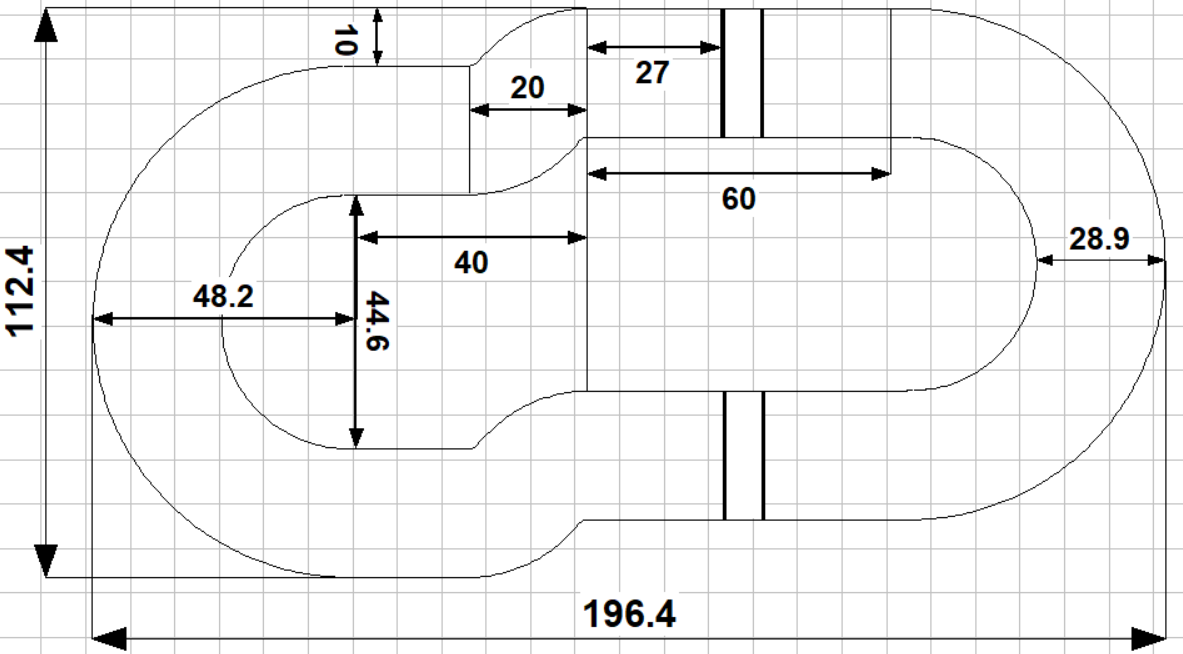
\includegraphics[width=0.8\textwidth]{Images/Tracks/Track1.PNG}
    \caption{Track 1 Layout in cm}
\end{figure}

\todo{Insert Final layout}








%\subsection{2. Prototype - Bus stop procedure}
%The second component is focused on detecting and performing a bus stop, and is built using the component of the steering object. 

%Using the requirements, this component needs to:\\
%    - Detect Bus Stops\\
%    - Stop parallel to the curb\\
%    - Stop within 1 cm of the curb

%The track will need to have some bus stops build on it, and it will also need to have some way to signal to the bus that a bus stop is coming up. This will most likely be a coloured piece of tape, that the bus will recognise with a LEGO colour sensor.\info{This is at least the plan as of this moment.}  Furthermore the track will also have to be circular to allow for the bus to keep driving around on the track and make repeated stops at the bus stops.



\subsection{2. Iteration - Bus stop procedure \& Speed Controller}
Intro: beskriv curb/bus stop procedure


\textbf{Bus stop procedure} \newline

\textbf{Speed Controller} \newline


\textbf{Track requirements} \newline
The redesigned track for the second iteration can be seen on figure.\todo{some stuff to fix here} %\ref{Track2Layout}.
The track is quite similar to the first track, however in this iteration the track contains a bus stop, and is connected so it's infinite. Furthermore the aspect ratio have been changed slightly to fit the redesigned bus, that means the minimal turning radius and lane width have been recalculated as described in appendix \ref{laneCalculations}. Lastly the track contains three new tape colours placed between the two lane tapes. The three colours are to be used with the nxt color sensor to detect incoming bus stops, and to determine the speed limit of the road.

The new requirements for the track is therefore as follows:
\begin{itemize}
  \item Detect Bus Stops
  \item Stop parallel to the curb(tape)
  \item Stop within 1 cm of the curb(tape)
  \item Stop so the bus sign is 1cm from the right corner of the bus
  \item Red tape to illustrate an incoming bus stop
  \item Green tape to illustrate high speed zone(Major Highway)
  \item Blue tape to illustrate low speed zone(Street)
\end{itemize}

\begin{figure}[H]
    \label{Track2Layout}
    \centering
    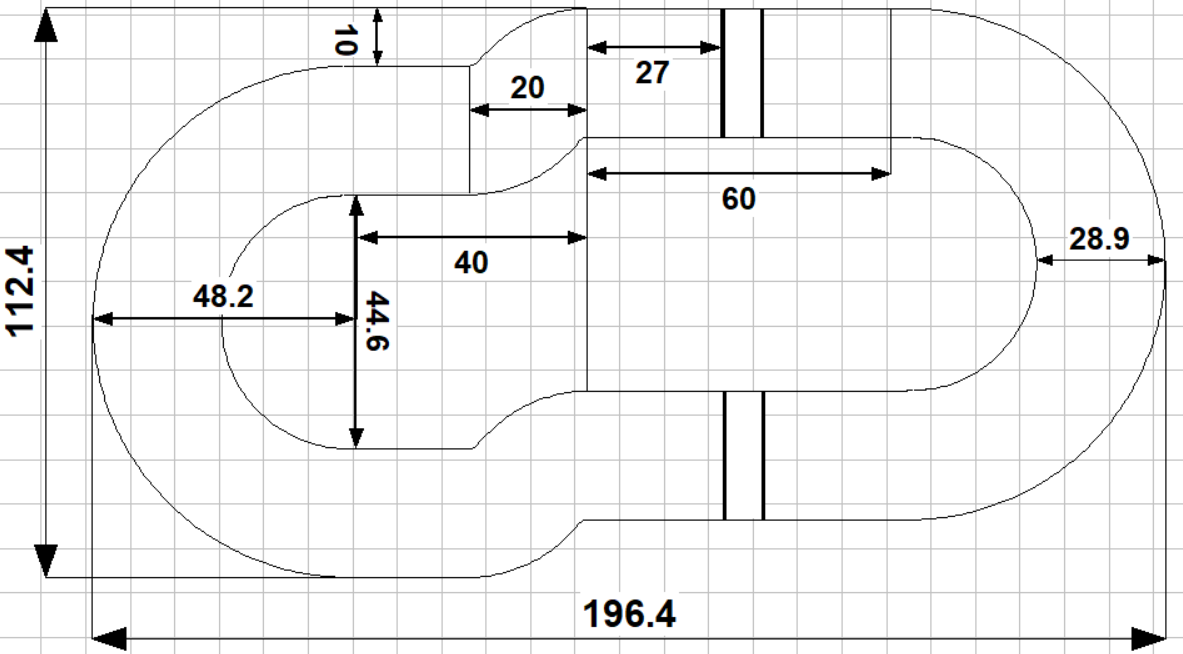
\includegraphics[width=0.8\textwidth]{Images/Tracks/Track1.PNG}
    \caption{Track 2 Layout in cm}
\end{figure}

\textbf{Bus Reconstruction} \newline
The redesigned bus can be seen on figure \ref{busDesign2}\todo{Missing picture of bus to reference}. The bus was redesigned to fix a couple of issues which was found upon testing in the first iteration.

\begin{itemize}
  \item Rear wheels felt off after the bus had driven for some time
  \item Unbalanced weight, which made it hard for the bus to turn left, but not right.
  \item The width and depth of the bus was not consistent, e.g. the ultrasonic sensor was placed too far in front. 

\end{itemize}

insert billede.












%OLD:
%As previously mentioned
%\ref{solvingRequirements
%\todo{fix}, we intend wish to detect a physical object emulating a sign and not just a drawing on the tracks. Towards this end we will be attempting to use a NXT CamV4 Sensor and some image recognition algorithm. 


%The bus scale should be a close approximate of a real bus scale as \cite{DriveingCurves}, 
%\subsection{3. Prototype - Cruise Control, BT stop button, obstacle safety protocol}
%\subsection{4. Prototype - Detecting bus stops}